% mnras_template.tex 
%
% LaTeX template for creating an MNRAS paper
%
% v3.0 released 14 May 2015
% (version numbers match those of mnras.cls)
%
% Copyright (C) Royal Astronomical Society 2015
% Authors:
% Keith T. Smith (Royal Astronomical Society)

% Change log
%
% v3.2 July 2023
%	Updated guidance on use of amssymb package
% v3.0 May 2015
%    Renamed to match the new package name
%    Version number matches mnras.cls
%    A few minor tweaks to wording
% v1.0 September 2013
%    Beta testing only - never publicly released
%    First version: a simple (ish) template for creating an MNRAS paper

%%%%%%%%%%%%%%%%%%%%%%%%%%%%%%%%%%%%%%%%%%%%%%%%%%
% Basic setup. Most papers should leave these options alone.
\documentclass[fleqn,usenatbib]{mnras}

% MNRAS is set in Times font. If you don't have this installed (most LaTeX
% installations will be fine) or prefer the old Computer Modern fonts, comment
% out the following line
\usepackage{newtxtext,newtxmath}
% Depending on your LaTeX fonts installation, you might get better results with one of these:
%\usepackage{mathptmx}
%\usepackage{txfonts}
\usepackage{listings}

% Use vector fonts, so it zooms properly in on-screen viewing software
% Don't change these lines unless you know what you are doing
\usepackage[T1]{fontenc}

% Allow "Thomas van Noord" and "Simon de Laguarde" and alike to be sorted by "N" and "L" etc. in the bibliography.
% Write the name in the bibliography as "\VAN{Noord}{Van}{van} Noord, Thomas"
\DeclareRobustCommand{\VAN}[3]{#2}
\let\VANthebibliography\thebibliography
\def\thebibliography{\DeclareRobustCommand{\VAN}[3]{##3}\VANthebibliography}


%%%%% AUTHORS - PLACE YOUR OWN PACKAGES HERE %%%%%

% Only include extra packages if you really need them. Avoid using amssymb if newtxmath is enabled, as these packages can cause conflicts. newtxmatch covers the same math symbols while producing a consistent Times New Roman font. Common packages are:
\usepackage{graphicx}	% Including figure files
\usepackage{amsmath}	% Advanced maths commands

%%%%%%%%%%%%%%%%%%%%%%%%%%%%%%%%%%%%%%%%%%%%%%%%%%

%%%%% AUTHORS - PLACE YOUR OWN COMMANDS HERE %%%%%

% Please keep new commands to a minimum, and use \newcommand not \def to avoid
% overwriting existing commands. Example:
%\newcommand{\pcm}{\,cm$^{-2}$}	% per cm-squared

%%%%%%%%%%%%%%%%%%%%%%%%%%%%%%%%%%%%%%%%%%%%%%%%%%

%%%%%%%%%%%%%%%%%%% TITLE PAGE %%%%%%%%%%%%%%%%%%%

% Title of the paper, and the short title which is used in the headers.
% Keep the title short and informative.
\title[vis-r]{\texttt{vis-r}: Quick radial profile modelling for interferometric visibilities}

% The list of authors, and the short list which is used in the headers.
% If you need two or more lines of authors, add an extra line using \newauthor
\author[G. M. Kennedy]{
Grant M. Kennedy$^{1}$\thanks{E-mail: g.kennedy@warwick.ac.uk}
\\
% List of institutions
$^{1}$Department of Physics, University of Warwick
}

% These dates will be filled out by the publisher
\date{Accepted XXX. Received YYY; in original form ZZZ}

% Enter the current year, for the copyright statements etc.
\pubyear{2024}

% Don't change these lines
\begin{document}
\label{firstpage}
\pagerange{\pageref{firstpage}--\pageref{lastpage}}
\maketitle

% Abstract of the paper
\begin{abstract}
This paper describes a method for parametric radial profile modelling of interferometric visibility data. Image-based parametric modelling is common in the field of circumstellar debris disks, and high resolution ALMA observations make this method computationally expensive because many high resolution images must be generated, Fourier transformed, and interpolated. Most debris disks are axisymmetric, so here a method that avoids generating images and instead models radial profiles is outlined. The two ideas that enable this method are i) $u,v$ space visibility averaging, and ii) using the Discrete Hankel Transform to convert arbitrary parametric radial surface brightness profiles to visibilities. Vertical scale height can be included, but is fixed with radius; in principle this is a limitation but in practise radially-dependent vertical structure information is beyond even ALMA's capability for all but a few debris disks. Combined, these ideas yield a method that is about two orders of magnitude faster than image based methods and can be run on a laptop, is sufficient for most ALMA observations of debris disks, and can be used with gradient-based fitting/sampling methods such as Hamiltonian Monte-Carlo.
\end{abstract}

% Select between one and six entries from the list of approved keywords.
% Don't make up new ones.
\begin{keywords}
keyword1 -- keyword2 -- keyword3
\end{keywords}

%%%%%%%%%%%%%%%%%%%%%%%%%%%%%%%%%%%%%%%%%%%%%%%%%%

%%%%%%%%%%%%%%%%% BODY OF PAPER %%%%%%%%%%%%%%%%%%

\section{Introduction}

Interferometry is a commonly used tool in astronomy. It circumvents problems that arise from the desire to have high angular resolution at a reasonable price point, but at the cost of added complexity for the end user; ``fringe visibility` is not a term that endears new users, nor is the prospect of developing methods that convert Fourier amplitudes to images, or vice versa.

The complexity of interferometric data, and the accessibility of facilities such as the Atacama Large Millimeter/submillimeter Array (ALMA), has driven the development of methods and software that aids the end user. For example, the \textsc{galario} package \citep{2018MNRAS.476.4527T} takes an input sky image, and given a list of antenna baseline coordinates and visibilities can return a $\chi^2$ goodness of fit metric that aids minimisation and sampling. Modelling data then becomes simpler for the end user, who can focus on generating images, for example with radiative transfer packages \citep[e.g. RADMC,][]{2012ascl.soft02015D} or more analytic methods \citep[e.g.][]{2021MNRAS.504.4497C}. Indeed, in the field of circumstellar debris disks, a workflow based around image generation and Markov Chain Monte Carlo (MCMC) sampling for parametric modelling of ALMA data has become the de facto standard.

However, there are downsides to this approach. Longer  baselines and consequent greater spatial resolution requires higher resolution images. But users typically also desire minimal flux loss, so obtain data that also has relatively short baselines.  Combined, the observational strategy means that model images must be large to contain low frequency information, but have small pixels to include high frequencies. Likewise the two-dimensional Fourier transforms of these images are large to cover high frequencies, and have many pixels so that low frequencies are sampled properly. For long-baseline datasets the requirement can be that the images are 8192 pixels on a side (i.e. $2^{13}$ to enable Fast Fourier Transforms). For a typical circumstellar disk most of these images can be empty because there is no structure on the largest scales, but the full images must nonetheless sit in computer memory, be Fourier transformed, and interpolated to compare with the observed data. Other more technical issues can be that i) fitting may not use gradient information to improve convergence and sampling efficiency, and ii) fitting is done in parallel, which may lead to significant demands on computer memory and/or require expensive many-core computing resources. While the computational resources used in fitting parametric models are not normally documented, servers with many tens of cores are the typical weapon of choice, and fitting runs can take sizeable fractions of a day for high resolution ALMA data. These issues could potentially be addressed by faster methods, and/or more analytic methods that can implement automatic differentiation, which would enable faster and more efficient fitting.

This article outlines a method that circumvents the aforementioned problems, providing a way to model radial profiles of axisymmetric structures for high resolution interferometric datasets. There are two key ideas; one is that radial profiles can be converted to visibilities with the Discrete Hankel Transform \citep[DHT,][]{2015JOSAA..32..611B}.\footnote{The reverse is also true; the the \textsc{frank} code described by \citet{2020MNRAS.tmp.1491J} uses the DHT to rapidly convert observations to radial profiles.}  While modelling radial profiles with the Hankel Transform is not new \citep[e.g.][]{2018ApJ...869L..48G}, use of the DHT is to this author's knowledge novel for forward modelling of radial profiles, and reduces the Hankel Transform integral to a matrix multiplication which is simpler and faster. The second idea is that given the ability to model the visibilities directly, $u,v$ averaging of observed visibilities becomes a key expedient. While the goal here is primarily to outline the approach, a small body of code has been written as a demonstration and is dubbed \textsc{vis-r}. An implementation in \textsc{python} can be run on high-resolution ALMA datasets on a laptop in a few minutes.

\section{Methods}

This section outlines the recipe for the fast radial profile modelling of visibilities. In what follows the 860\,$\mu$m ALMA observations of HR~4796 analysed by \citet{2018MNRAS.475.4924K} are used for illustrative purposes. The data show an inclined narrow ring with a radius of 1.1\arcsec. The self-calibrated data were used, and the raw data initially averaged to four channels with time bins of 30\,s, resulting in 321,322 visibilities.

\subsection{Visibility averaging}\label{sec:avg}

The idea of binning visibilities is not new. The typical averaging approach is to average over time and frequency; this preserves the data structure, and can reduce the volume significantly to yield products that can be distributed for continuum modelling. For modelling via images and Fourier transforms this averaging method is sufficient as image generation is normally the most expensive step. However, for the approach outlined here to be fast, averaging in $u,v$ space (i.e. sky-projected baseline length$/\lambda$ space) is done, which removes the time and frequency dimensions completely and can reduce the visibility data volume by one to two orders of magnitude without a serious loss of information.

In averaging, individual $u,v$ points must not be combined too enthusiastically, which results in ``beam smearing''. This effect can be quantified in terms of flux loss for a point source some distance $\Delta \theta$ from the phase center, the phase shift between frequency-averaged channels must be limited such that the parameter $\beta$ is small, where
\begin{equation}
    \beta = \frac{\Delta \theta}{\theta_{\rm s}} \frac{\Delta \nu}{\nu}
\end{equation}
where $\theta_{\rm s}$ is the synthesised beam size, $\nu$ is frequency, $\Delta \nu$ is the range of frequencies being averaged. For a 1\% decrement in flux for a point source at $\Delta \theta$, $\beta \approx 0.14$ \citep{1989ASPC....6..247B}.\footnote{See also \href{https://safe.nrao.edu/wiki/pub/Main/RadioTutorial/BandwidthSmearing.pdf}{https://safe.nrao.edu/wiki/pub/Main/RadioTutorial/BandwidthSmearing.pdf}.} Using $\theta_{\rm s} \approx \lambda/b$, this equation can be rewritten as
\begin{equation}\label{eq:avg1}
    \beta \approx \Delta \theta \left[ \frac{\Delta \nu}{\nu} \frac{b}{\lambda} \right] \, .
\end{equation}
The typical application of this equation is to take $b$ as the maximum baseline in the dataset and $\Delta \theta$ as the primary beam half-width at half-maximum (i.e. the outer ``edge'' of the data). Given the average frequency of the dataset, $\Delta \nu$ is then fixed and the data averaged to a smaller number of frequency channels.

However, this averaging is conservative; if the maximum baseline were halved (e.g. the longer baseline data discarded), then the frequency averaging could be more aggressive because $\Delta \nu$ can be doubled. This more aggressive averaging keeps the term in parentheses in equation~(\ref{eq:avg1}) constant, rather than $\Delta \nu$ constant. As $u,v = b/\lambda$, the term in parentheses can then be seen as a constant radial distance in $u,v$ space over which averaging is done, $\Delta_{u,v}$, for a given $\beta$, so we can instead write
\begin{equation}\label{eq:avg2}
    \Delta_{u,v} \approx \frac{1}{\beta \, \Delta \theta} \, .
\end{equation}

The same idea applies to time averaging, but the details differ \citep{1989ASPC....6..247B}. However, with the criterion that the rotation does not move the offset point source by a sizeable fraction of the synthesised beam, the result is that the $\Delta \nu / \nu$ in equation (\ref{eq:avg1}) is replaced by $\Delta t / P$, where $\Delta t$ is the averaging window and $P$ the Earth's sidereal period ($\approx$24\,h). Thus, time averaging can also be seen as setting a $\Delta_{u,v}$ criterion.

One can therefore reduce the data volume by binning visibility data in $u,v$ space with a constant bin size $\Delta_{u,v}$. This is in contrast to the typical approach where data are time and frequency averaged, which effectively has a bin size that decreases with $u,v$. Because the density of baselines in $u,v$ space is higher for smaller $u,v$, the former approach can reduce the number of visibilities being fit during modelling drastically, without any loss of fidelity. While this reduction may have little effect for image-based modelling, where generating images is commonly the most expensive step, it is a key expedient when modelling the visibilities directly.

To be clear, the above ``derivation'' is heuristic, not quantitative. Users should experiment for their particular case, verifying that the results do not change as $\Delta_{u,v}$ is decreased. An example case is given below, for which $\Delta \theta \gtrsim 2r$, where $r$ is the radius of an annular disk, was found to be sufficient.

\begin{figure}
    \centering
    \hspace{-0.5cm}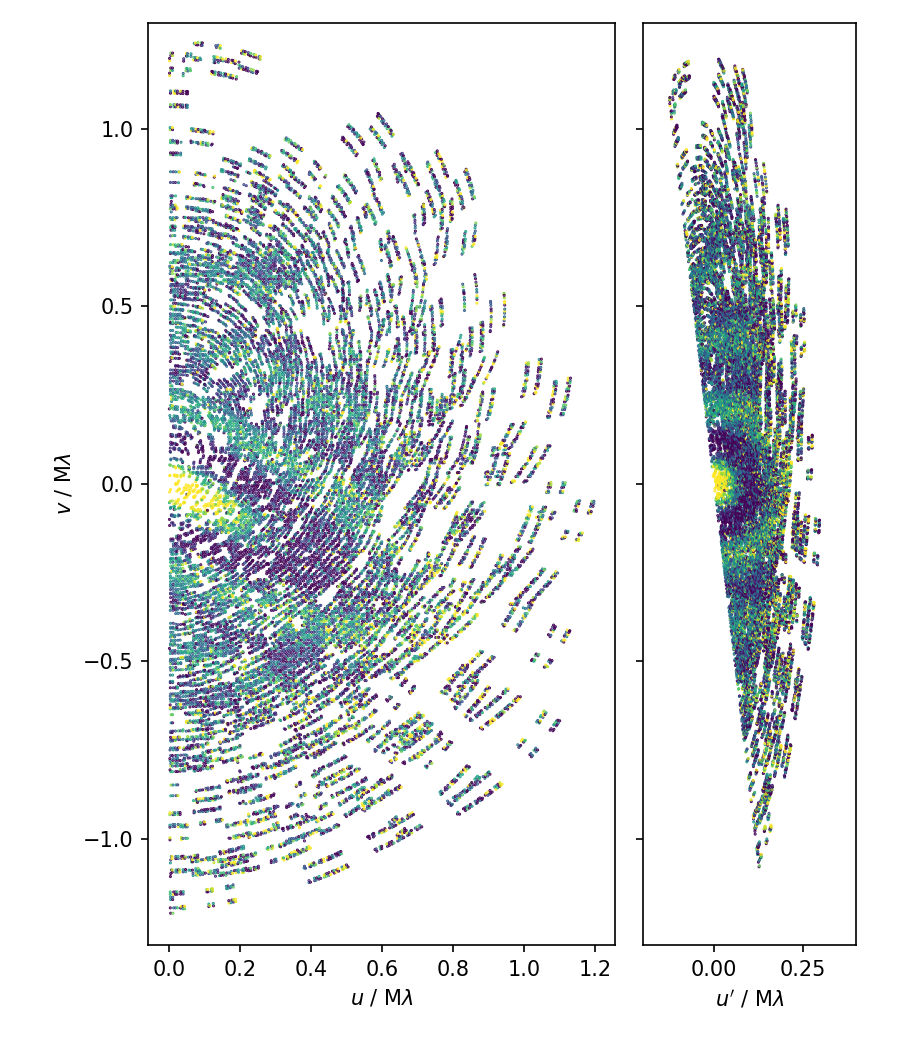
\includegraphics[width=0.5\textwidth]{vis_avg.png}
    \caption{Visibility binning and transformation for HR~4796 data, each point is a baseline that is coloured by the real component of the visibility in the range -0.005 to 0.01\,Jy. The left panel shows the binned visibilities with $\Delta_{u,v}=7350$, and the right panel shows them after rotation and shrinking given the disk position angle and inclination. The coordinates are compressed by a factor 0.24 along the rotated $u$ axis because the disk is highly inclined. The visibility pattern is circular in the right panel, so can be modelled purely in terms of the radial dependence about the origin.}
    \label{fig:bin}
\end{figure}

In practise this binning is a weighted sum of the baseline lengths $u$ and $v$ and visibilities $V$ that fall in a given bin (i.e. $\bar{x} = \Sigma x_j w_j / \Sigma w_j$). The weights $w$ in a bin are themselves summed, as they are the inverse variance for a given visibility. Baselines with negative $u$ can be rotated by 180$^\circ$, and their visibilities complex conjugated before binning, which further reduces the number of binned visibilities. An illustration of the binned visibility coordinates is shown in the left panel of Figure \ref{fig:bin} for $\Delta_{u,v}=7350$. The number of visibilities in this case has been reduced from 321,322 to 19,493.

\subsection{Radial profile modelling}

This section outlines how to model a set of visibilities for a given input radial profile. Here the model will be called a ``disk'', primarily because this model has been developed for modelling of debris disks observed with ALMA, but could be any asisymmetric structure. The radial profile will necessarily be parameterised with the goal of deriving best-fit values and uncertainties for those parameters. The model could in principle be the surface brightness of a series of radial locations, but for extracting empirical radial profiles other methods are far better suited, most notably \textsc{frank} \citep{2020MNRAS.tmp.1491J}. \textsc{frank} uses the Discrete Hankel Transform to quickly convert a set of visibilities into a radial profile; the method here is essentially the opposite, converting a profile radial profile to visibilities with the DHT for comparison with the data. See \citet{2020MNRAS.tmp.1491J} for a detailed discussion of the DHT and how it is used. Here, we simply need the transform, which is
\begin{equation}\label{eq:dht}
    \Tilde{f}(q_{\rm k}) = \boldsymbol{Y}_{\rm f} \, f(r_{\rm k}, p) \, ,
\end{equation}
where $\Tilde{f}$ is the set of model visibilities, $\boldsymbol{Y}_{\rm f}$ is a $N \times N$ matrix of coefficients, and $f$ is the input radial surface brightness profile given some parameters $p$. Typically $p$ will contain geometric parameters that are common to every model (position angle $\phi$, inclination $i$, and sky offsets $\Delta \alpha$, $\Delta \delta$), and disk-specific parameters that dictate the surface brightness or total flux, shape, and scale of the profile (e.g. Gaussian location $r_0$ and width $\sigma_{\rm r}$). The profile is computed at a specific set of $N$ radial ``collocation'' points $r_{\rm k}$, that have corresponding points in $u,v$ space $q_{\rm k}$.

While the model normalisation could be done with a parameter that specifies the surface brightness (e.g. at $r_0$), in practise it is better to use this parameter to specify the total flux on the shortest baseline $\Tilde{f}(q_0)$. This quantity will vary little from model to model and is only weakly correlated with other model parameters.

Practically, two parameters are specified in setting up the DHT. One is $R_{\rm out}$, which is the radius beyond which the radial profile is zero (i.e. the maximum spatial scale, or the lowest spatial frequency $q_1$). The $q_k$ are given by $q_k = j_{0k}/(2 \pi R_{\rm out})$, where $j_{0k}$ is the $k$th zero of the zeroth-order Bessel function, $J_0(j_{0k}=0$). The second parameter is $N$, the number of collocation points, which for fixed $R_{\rm out}$ sets the highest spatial frequency ($q_{\rm N}$). 

The interpolation step below means that values for $R_{\rm out}$ and $N$ should be chosen so that the collocation points span the range of $u,v$ baseline lengths $q_{u,v}$. Typically $R_{\rm out}$ will therefore be larger than the radius beyond which the model has zero flux. The range of $q_{u,v}$ however depends on the inclination of the model, so if $R_{\rm out}$ is fixed for an entire fitting/sampling run where inclination may vary, then some care is needed. Practically, $R_{\rm out}$ can be found given an initial estimate of the disk inclination from $R_{\rm out} = j_{01}/(2 \pi \min{(u,v)} \cos i)$. Then the number of collocation points $N$ found with $j_{0N}/(2 \pi R_{\rm out}) > \max{(\sqrt{u^2+v^2})}$.

For disk modelling the geometry is typically parameterised as a position angle $\phi$ (East of North) and inclination $i$. To account for an inclined disk the model $u,v$ distances could be radially stretched along the disk minor axis, to account for the smaller spatial scale (greater spatial frequencies). In practise however, the model is purely radial so the observed $u,v$ distances are instead squeezed. This transform is therefore achieved with a rotation and scaling of the observed visibilities at coordinates $u,v$ \citep[e.g. as in][]{2018MNRAS.476.4527T}, given by
\begin{gather}
    u' = u \cos \phi - v \sin \phi \notag \\
    v' = u \sin \phi + v \cos \phi
\end{gather}
and 
\begin{equation}
    q_{\rm u,v} = \sqrt{[u' \cos i]^2 + v^2} \, .
\end{equation}
The result of this transformation, before the hypotenuse is calculated, is shown in the right panel of Figure \ref{fig:bin}.

Given these transformed radial $u,v$ coordinates, the model is interpolated to obtain model visibilities for every observed baseline
\begin{equation}
    \Tilde{f}(q_{\rm k}) \rightarrow \Tilde{f}(q_{\rm u,v}) \, .
\end{equation}
A comparison of a radial model with the observed visibilities is shown in Figure \ref{fig:model}. $R_{\rm out}=30$\arcsec~is used, as the disk inclination of 76$^\circ$ means that the minimum $q_{\rm u,v}$ is shrunk by a factor of four relative to a face-on disk. The model is a narrow annulus, and in fact has little flux beyond 1.1\arcsec.

\begin{figure}
    \centering
    \hspace{-0.5cm}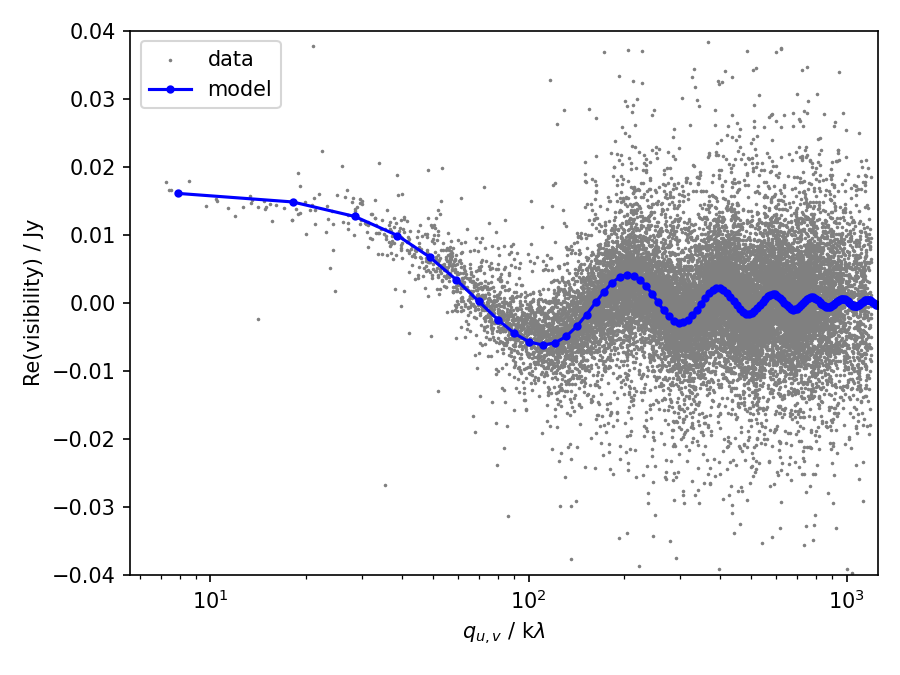
\includegraphics[width=0.5\textwidth]{model.png}
    \caption{Model and binned data in radial visibility coordinates, with $R_{\rm out} = 30$\arcsec~and $N=380$.}
    \label{fig:model}
\end{figure}

The penultimate step is to incorporate vertical structure. For optically thin disks this step is absolutely necessary, as inclined disks are brightened at their ansae by the longer line of sight through the disk. In image space, a constant absolute scale height for a Gaussian distribution can be implemented with a 1-d convolution along the disk minor axis. The dispersion of the Gaussian is $\sin i$ times the real vertical dispersion to account for the disk inclination (i.e. a face-on disk has no ansae brightening). The properties of Fourier transforms mean that this Gaussian convolution is an exponential multiplication of the ``flat'' interpolated model in Fourier space;
\begin{equation}\label{eq:vert}
    \Tilde{f}(q_{\rm u,v})' = \Tilde{f}(q_{\rm u,v}) \, \exp{(-[2 \pi (z_{\rm h} r_0 \sin i) \, u']^2/2)}
\end{equation}
where $z_{\rm h}$ is the relative scale height at some representative disk radius $r_0$.

Typically it is assumed that the  vertical distribution in a disk is Gaussian, and that the height varies as a function of stellocentric radius, for example dust particles that have a fixed inclination. Here however the scale height $H$ is constant simply because it can be modelled analytically. In practise our ability to quantify the scale height dependence is limited, so this choice is not a serious limitation. For example, \citet{2023MNRAS.524.1229T} find that for 49~Ceti, while a constant relative scale height is preferred (i.e. $H/r=$ constant), a constant absolute height is consistent with the ALMA data at the 2$\sigma$ level. As noted by \citet{2023MNRAS.524.1229T}, this disk is one of the most promising for quantifying the radial dependence of scale height. Thus, while not necessarily what one would choose given total freedom, the constant absolute vertical profile should be sufficient for all but the highest resolution data for the broadest disks.

Finally, the model can be translated to account for any offset of the disk from the observation phase center. This is simply a phase shift (rotation into the complex plane) of the model visibilities using the original binned $u,v$ coordinates $\gamma = u \Delta \alpha + v \Delta \delta$.
\begin{equation}\label{eq:phase}
    \Tilde{f}(q_{\rm u,v})'' = \Tilde{f}(q_{\rm u,v})' \, \exp{(2 \pi \iota \gamma)}
\end{equation}
where here $\iota = \sqrt{-1}$.

In summary, the procedure to compare a model with parameters $p$ with data is to choose $R_{\rm out}$ and $N$, obtain the radial profile at $r_{\rm k}$, apply the DHT (equation [\ref{eq:dht}]) to get $\Tilde{f}(q_{\rm k})$. The binned observational baseline coordinates are transformed to find $q_{u,v}$, and then used to interpolate $\Tilde{f}(q_{\rm k})$ at $q_{u,v}$. This model is then multiplied by the exponential in equation (\ref{eq:vert}) to add the vertical dimension. The model is shifted some distance from the phase center to obtain the final model $\Tilde{f}(q_{u,v})''$. This model can then be compared with the data, e.g. by computing a sum of squared differences. To visualise how well the model fits the data, the model can be interpolated at the original unbinned $u,v$ locations and subtracted from the data, which can then be imaged.

\subsection{Verification}

As proof of concept some example results are given for implementations in \textsc{python} and \textsc{stan} \citep{2017JSS....76....1C}, with the goals of showing that the results are equivalent to those obtained with an imaging code \citep[e.g.][]{2021MNRAS.504.4497C}, and illustrating the effect of visibility averaging. A few more notes on implementation are given in the Appendix.\footnote{Examples of the \textsc{stan} and \textsc{python} implementations are available at \href{https://github.com/drgmk/vis-r}{https://github.com/drgmk/vis-r}.}


The HR~4796 ALMA dataset is modelled with a 3-dimensional Gaussian torus that has parameters $\Delta \alpha$, $\Delta \delta$ (sky offsets), $\phi$, $i$ (position angle and inclination), $F$ (flux), $r_0$, $\sigma_{\rm r}$, and $h$ (disk radius, width and scale height). These parameters are the same between models, with the exception that $f$ is total flux for image modelling and the flux on the shortest baseline for visibility modelling, and $h$ is relative $H/r$ for image modelling and absolute $H/r_0$ for visibility modelling. The visibility data are averaged as above, with $\Delta_{u,v} = 7350$. The dataset here has a 0.17\arcsec~beam, which is at the higher end of what is possible with ALMA for debris disks, which are typically limited by surface brightness. The disk is about 1\arcsec~in radius, which is relatively small. 

Two tests are done. The first is to compare the posterior distributions for the three models, and the second to compare posterior distributions across different levels of $u,v$ binning.

\begin{figure}
    \centering
    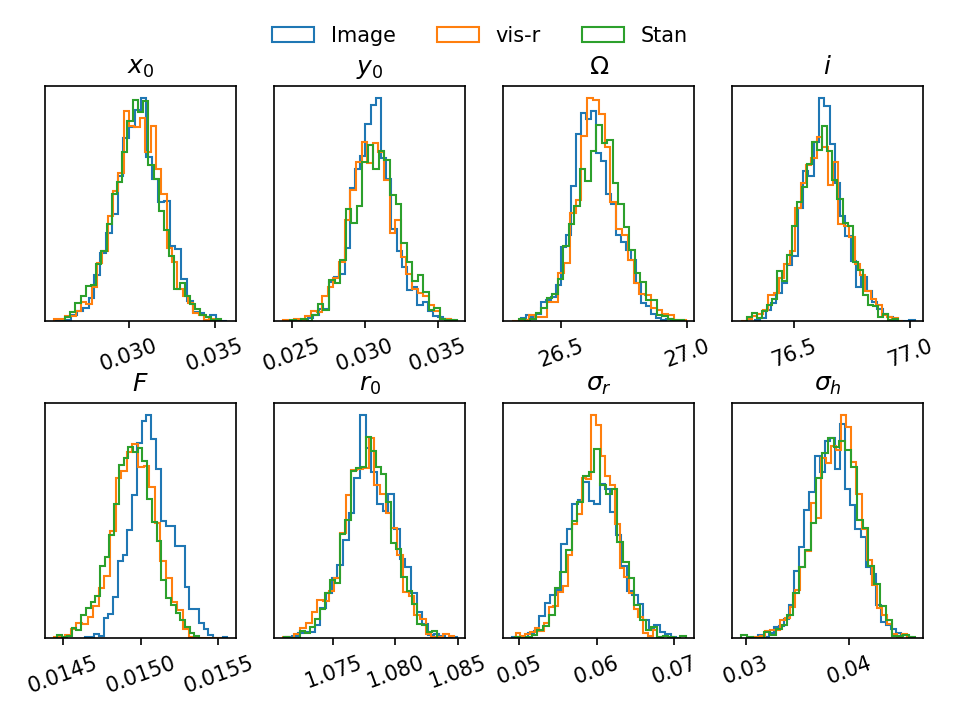
\includegraphics[width=0.5\textwidth]{comp.png}
    \caption{Comparison among image and visibility based posterior distributions for the HR~4796 dataset. Units are seconds of arc, Jansky, and degrees. The only significant difference is that the visibility method yields a lower average $F$ parameter, because for this method $F$ is the flux on the shortest baseline, while for the imaging method $F$ is the total disk flux.}
    \label{fig:comp}
\end{figure}

Figure \ref{fig:comp} shows posterior distributions of the eight disk model parameters for the three models. The only difference is that for the $F$ parameter the visibility model fluxes are a few percent lower because the shortest baseline is non-zero. Thus, the visibility model is capable of producing equivalent results without generating images. Cases where the radial scale height dependence is strongly constrained in the data will require an image-based method, but as noted above these will be rare.

To give a feel for the speed of these methods, the time taken for one model likelihood evaluation with this dataset on an M2 MacBook Air in \textsc{python} is about 50\,ms for the imaging code. The visibility based method in \textsc{python} takes about 1\,ms, so is significantly faster. With no binning of visibilities this time increases to about 25\,ms, illustrating why binning is beneficial. In \textsc{stan} a single evaluation with the visibility method takes 14\,ms, but bear in mind that this time includes calculation of the gradients ($d \chi^2 / dp_i$), and that convergence is much faster and fewer samples are needed to build posteriors. Full fitting runs take minutes for \textsc{vis-r}, and do not change strongly with dataset. For the image-based method the time taken depends strongly on the resolution of the data, and can take from tens of minutes to around half a day. The speed of the imaging code can be improved up to a point by $u,v$ binning, but image creation eventually becomes the bottleneck, at which speed increases come from lower resolution images. The visibility codes depend mainly on the level of visibility averaging, with the most time spent on transformation of the visibility coordinates and interpolation.

\begin{figure}
    \centering
    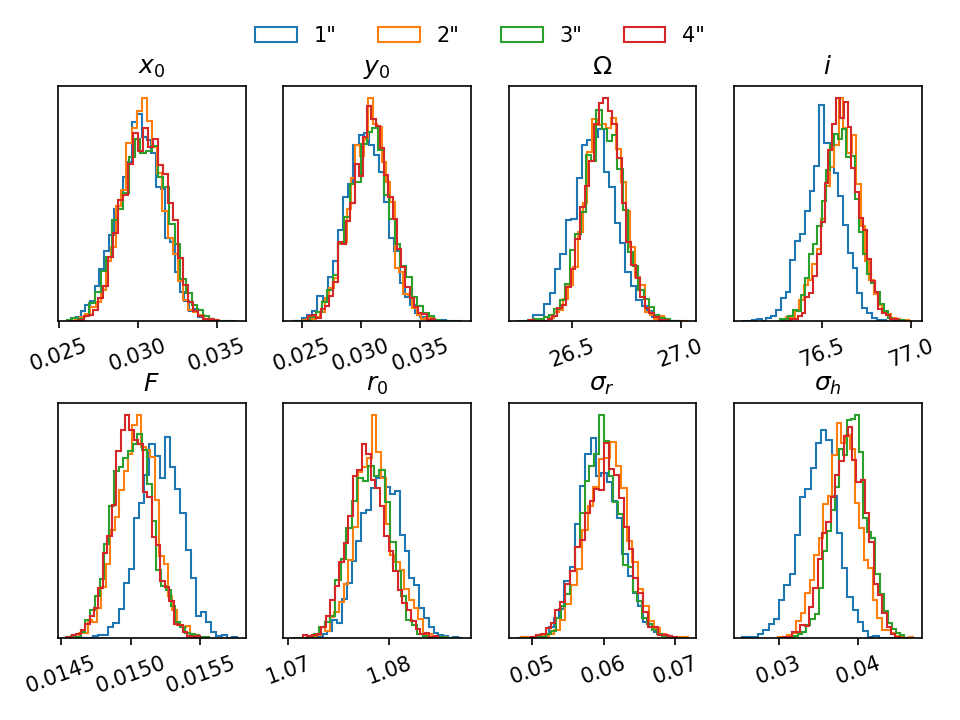
\includegraphics[width=0.5\textwidth]{avg.png}
    \caption{Effect of visibility averaging levels; the disk here is 1\arcsec~in radius. Averaging on the scale of the disk lowers the model flux, but only a few percent. Units are seconds of arc, Jansky, and degrees.}
    \label{fig:avg}
\end{figure}

A second comparison is among different levels of averaging, as shown in Figure \ref{fig:avg}. The averaging here has been cast in terms of seconds of arc, using equation \ref{eq:avg2} with $\beta=0.14$. It is clear from the posteriors that averaging to a spatial scale that is the same radius as the disk is somewhat detrimental, but only the flux is strongly affected, and only at the few percent level. Reliable initial parameter estimates can therefore be quickly obtained with fairly hard averaging.

\section{Summary}

This paper outlines a method for the rapid radial profile modelling of interferometric data, dubbed \textsc{vis-r}. The enabling ideas are visibility averaging in $u,v$ space and the Discrete Hankel Transform to convert model profiles into visibilities. Aside from cases where vertical structure is key, \textsc{vis-r} yields results that are equivalent to much more complex and computationally expensive image-based methods.

\section*{Acknowledgements}

The method outlined here is inspired by \textsc{frank} \citep{2020MNRAS.tmp.1491J} and the data produced by the ALMA Large Programme ARKS. GMK is supported by the Royal Society as a Royal Society University Research fellow..

%%%%%%%%%%%%%%%%%%%%%%%%%%%%%%%%%%%%%%%%%%%%%%%%%%
\section*{Data Availability}

This paper makes use of the following ALMA data: ADS/JAO.ALMA\#2015.1.00032.S ALMA is a partnership of ESO (representing its member states), NSF (USA) and NINS (Japan), together with NRC (Canada), MOST and ASIAA (Taiwan), and KASI (Republic of Korea), in cooperation with the Republic of Chile. The Joint ALMA Observatory is operated by ESO, AUI/NRAO and NAOJ.

%%%%%%%%%%%%%%%%%%%% REFERENCES %%%%%%%%%%%%%%%%%%

% The best way to enter references is to use BibTeX:

\bibliographystyle{mnras}
\bibliography{ref} % if your bibtex file is called example.bib


% Alternatively you could enter them by hand, like this:
% This method is tedious and prone to error if you have lots of references
%\begin{thebibliography}{99}
%\bibitem[\protect\citeauthoryear{Author}{2012}]{Author2012}
%Author A.~N., 2013, Journal of Improbable Astronomy, 1, 1
%\bibitem[\protect\citeauthoryear{Others}{2013}]{Others2013}
%Others S., 2012, Journal of Interesting Stuff, 17, 198
%\end{thebibliography}

\appendix

\section{Notes on implementation}

The method can be implemented in different ways. The most straightforward is as a log(probability) function that replaces an image-based one, for example within an MCMC script using \textsc{emcee} \citep{2013PASP..125..306F}. Averaging of the visibility data can be implemented with the \textsc{binned\_statistic\_2d} function in \textsc{scipy.stats}.

One potential advantage is that the method is sufficiently analytic that it can be implemented in codes that use automatic differentiation, and hence can benefit from gradient-based methods such as Hamiltonian Monte-Carlo (HMC). HMC uses gradients to sample the posteriors more efficiently, resulting in less correlation between samples and very little sample rejection, both of which mean fewer samples are needed to build good posteriors. However, HMC deals less well with strongly correlated posteriors and different parameter scales and must learn these during a ``warmup'' phase. This can be aided by scaling the parameter distributions to have unit variance and be centered about zero. Experience finds that this method can work very rapidly, but in some cases experimentation with the parameter scaling is needed to ensure the warmup phase proceeds quickly.

In contrast, \textsc{emcee} is extremely robust to parameter correlations and dynamic range. While convergence can be much slower, testing suggests that using an implementation in \textsc{python} with \textsc{emcee} (or similar) is likely to require less tuning, and hence overall a faster path to final fitting results.

% Don't change these lines
\bsp	% typesetting comment
\label{lastpage}
\end{document}

% End of mnras_template.tex
